% Chapter 5 — GPU-Based Storage I/O Optimizations  (31 pages, ~50-60 min)
% Style matches chapter06-presentation-v3.tex (Madrid/navy, \kw, \pe, \bridge).
% Script: chapter05-lecture-script-zh.md
% Compile: pdflatex chapter05-presentation.tex  (run twice)
\documentclass[aspectratio=169]{beamer}

% ====== Presenter info: EDIT ME ======
\newcommand{\PresenterName}{Tianqin Cai}          % <-- 改成你的名字
\newcommand{\PresenterTitle}{Applied Scientist} % <-- 改成你的头衔
\newcommand{\PresenterOrg}{AWS}
% =====================================

\usetheme{Madrid}
\definecolor{navy}{RGB}{18,47,90}
\definecolor{kwblue}{RGB}{0,56,132}
\definecolor{okgreen}{RGB}{80,130,20}
\usecolortheme[named=navy]{structure}
\setbeamercolor{frametitle}{bg=navy,fg=white}
\setbeamercolor{title}{bg=navy,fg=white}
\setbeamercolor{block title}{bg=navy,fg=white}
\setbeamercolor{block body}{bg=gray!12,fg=black}
\setbeamercolor{block title example}{bg=okgreen,fg=white}
\setbeamercolor{block body example}{bg=okgreen!10,fg=black}
\setbeamertemplate{navigation symbols}{}
\setbeamertemplate{blocks}[rounded][shadow=true]

\usepackage{booktabs}
\usepackage{listings}
\lstset{
  language=C++,
  basicstyle=\ttfamily\fontsize{6.5}{7.6}\selectfont,
  keywordstyle=\color{kwblue}\bfseries,
  commentstyle=\color{gray}\itshape,
  stringstyle=\color{okgreen},
  showstringspaces=false,
  breaklines=true,
  columns=fullflexible
}

\newcommand{\kw}[1]{\textbf{\textcolor{kwblue}{#1}}}
\newcommand{\pe}[1]{\par{\setlength{\fboxsep}{2.5pt}\noindent\colorbox{navy!9}{\parbox{\dimexpr\textwidth-5pt\relax}{\footnotesize\itshape Plain English: #1}}}}
\newcommand{\bridge}[1]{{\footnotesize\itshape\textcolor{gray}{#1}}\par}
\newcommand{\refmark}[1]{\textsuperscript{[#1]}}

\title[AI Systems Performance Engineering]{AI Systems Performance Engineering}
\subtitle{Chapter 5 --- GPU-Based Storage I/O Optimizations}
\author[\PresenterName\ \ \PresenterTitle\ \ \PresenterOrg]{\PresenterName\\\PresenterTitle\\\PresenterOrg}
\institute[]{\footnotesize Internal Training for Applied Scientists on AI Infrastructure}
\date{September 2026}

\begin{document}

% ================================================================ 1
\begin{frame}
  \titlepage
\end{frame}

% ================================================================ 2
\begin{frame}{Roadmap: Five Parts, Each Answers One Question}
  \begingroup\small\setlength{\tabcolsep}{6pt}\renewcommand{\arraystretch}{1.25}
  \begin{tabular}{@{}ll@{}}
    \toprule
    \textbf{Part} & \textbf{The question it answers} \\
    \midrule
    I \ Storage fundamentals & How do we \kw{lay out and read data} so disks deliver peak bandwidth? \\
    II \ Direct GPU data paths & How does data \kw{skip the CPU bounce buffer} on its way to HBM? \\
    III \ Shared storage at scale & What serves \kw{many nodes} without becoming the bottleneck? \\
    IV \ The data pipeline & How do \kw{loaders and preprocessing} keep every GPU fed? \\
    V \ Profiling workflow & Is the job \kw{I/O-, communication-, or compute-bound}? \\
    \bottomrule
  \end{tabular}\endgroup
  \bigskip
  \begin{block}{The whole chapter in one sentence}
    \centering \kw{Keep the data pipeline as full as the compute pipeline --- a starving GPU is a wasted GPU.}
  \end{block}
  \medskip
  \centering\footnotesize\itshape
  When a detail page appears (io\_uring, cuFile, 3FS, DALI\ldots), it always belongs to one of these five questions.
\end{frame}

% ================================================================ 3
\begin{frame}{Part I --- Feeding Data Is as Important as the Compute Itself}
  \begin{columns}[c]
    \column{0.58\textwidth}
    \begin{itemize}
      \item Picture a \kw{100-trillion-parameter} model training on thousands of GPUs over
            \kw{billions of samples} --- terabytes of text, petabytes of images.
      \item If the storage pipeline is slow, \kw{GPUs starve and sit idle} --- low utilization
            despite every network optimization from Chapter 4.
      \item This chapter: read data efficiently from disk or remote storage, preprocess it,
            and \kw{overlap its I/O with GPU compute}.\refmark{1}
    \end{itemize}
    \column{0.40\textwidth}
    \begin{block}{Sizing the appetite (book example)}
      \small Each GPU needs \kw{200 MB/s} of training data:\\[2pt]
      {\small\setlength{\tabcolsep}{4pt}
      \begin{tabular}{@{}ll@{}}
        \toprule
        8 GPUs & $\sim$\kw{1.6 GB/s} \\
        GB200 NVL72 (72 GPUs) & \kw{14--20 GB/s} \\
        \bottomrule
      \end{tabular}}\\[3pt]
      \footnotesize Heavier multimodal samples? Calibrate with \kw{measured}
      bytes-per-sample $\times$ samples-per-second --- demand can be much higher.
    \end{block}
  \end{columns}
  \pe{the world's finest kitchen plates nothing if the pantry line is empty --- feeding the factory is a job of its own.}
\end{frame}

% ================================================================ 4
\begin{frame}{Data Locality: Put the Data Physically Close to the Compute}
  \begin{columns}[t]
    \column{0.50\textwidth}
    \begin{itemize}\small
      \item ``Close'' = \kw{local NVMe SSD} on the node, or at least \kw{in-rack} via
            NVMe-over-Fabrics (\kw{NVMe-oF}) --- fewer network hops, more consistent performance.
      \item Network storage (NFS, Amazon S3)? Verify the \kw{aggregate read bandwidth}
            across all compute nodes covers the appetite from the last page.
      \item Parallel filesystems (Lustre, GPFS) can \kw{cache data on local SSDs}.
    \end{itemize}
    \column{0.46\textwidth}
    \begin{block}{Shard the dataset across nodes}
      \small 100 TB, 10 nodes $\Rightarrow$ \kw{presplit 10 TB} onto each node's local disk;
      each node's loader reads \kw{only its local shard} --- no redundant network reads.
    \end{block}
    \begin{itemize}\small
      \item PyTorch's \kw{\texttt{DistributedSampler}} coordinates workers so each process
            gets a \kw{unique slice} per epoch --- aligns perfectly with per-node sharding.
    \end{itemize}
  \end{columns}
  \pe{don't make every workshop order from the overseas warehouse --- stock each workshop's own shelf with the parts it will use.}
\end{frame}

% ================================================================ 5
\begin{frame}{Sequential Beats Random: Shard Your Samples}
  \begin{columns}[t]
    \column{0.52\textwidth}
    \begin{itemize}\small
      \item Storage delivers far higher throughput for \kw{large sequential reads} than for
            small random ones --- and GPUs want data in \kw{large contiguous chunks}.
      \item Anti-pattern: \kw{millions of individual image files} $\Rightarrow$ random seeks
            all over the disk.
      \item Instead: pack samples into a few \kw{large binary shards} --- Arrow, TFRecord,
            Parquet, WebDataset tar --- one read returns \kw{many samples}.
      \item Same on object stores: \kw{combine small S3 objects} into larger ones ahead of time.
    \end{itemize}
    \column{0.44\textwidth}
    \begin{block}{Tune the read size too}
      \small Reading in \kw{1 MB} chunks beats \kw{4 KB} chunks --- lower per-read overhead.
      Loader libraries expose \kw{buffer} and \kw{prefetch chunk} sizes; tune them even though
      the libraries are internally optimized.
    \end{block}
    \begin{itemize}\small
      \item Book warning: with today's faster GPUs, small random reads become the bottleneck
            \kw{sooner} --- verify your filesystem's small-read behavior explicitly.
    \end{itemize}
  \end{columns}
  \pe{pick up a full pallet per warehouse trip, not one screw at a time --- and pre-pack the screws into pallets before training starts.}
\end{frame}

% ================================================================ 6
\begin{frame}{When Reads Must Be Random: Parallelism and the Right Filesystem}
  \begin{columns}[t]
    \column{0.50\textwidth}
    \begin{block}{Hide latency with many in-flight reads}
      \small Issue \kw{multiple reads in parallel}: threads calling \texttt{pread()}, or Linux
      async I/O via \kw{\texttt{io\_uring}} --- preregistered buffers + polling submit
      \kw{batches of I/O} with minimal kernel overhead $\Rightarrow$ high IOPS.
    \end{block}
    \begin{itemize}\small
      \item Buffered I/O and big read-ahead help \kw{sequential} scans;
            random reads benefit little --- \kw{batch} them or use a dataset API
            (\texttt{TFRecordDataset}, \texttt{IterableDataset} + \texttt{DataLoader}).
    \end{itemize}
    \column{0.46\textwidth}
    \begin{block}{Filesystem choices (book tips)}
      \small
      \begin{itemize}\small
        \item \kw{XFS} is common on Linux NVMe servers; mount with \kw{\texttt{noatime}}
              --- no access-time write on every read.
        \item Amazon EFS: use \kw{Max I/O} performance mode; switch Bursting $\to$
              \kw{Provisioned throughput} for consistent bandwidth.
      \end{itemize}
    \end{block}
  \end{columns}
  \pe{if you must fetch single screws, send \kw{many runners at once} and stop stamping a timecard on every trip.}
\end{frame}

% ================================================================ 7
\begin{frame}{NVMe and Kernel Tuning: Scheduler, Read-Ahead, RAM}
  \begin{columns}[t]
    \column{0.52\textwidth}
    \begin{itemize}\small
      \item Modern Linux: multiqueue block I/O (\kw{blk-mq}) spreads I/O across cores.
            For NVMe use the \kw{none} or \kw{mq-deadline} scheduler (CFQ is obsolete);
            verify via \texttt{/sys/block/nvme*/queue/scheduler}.
      \item \kw{Read-ahead}: default $\sim$128 KB; streaming large files? raise to
            \kw{a few MB} (\texttt{blockdev --setra}) --- fewer syscalls, pipelined reads.
      \item Fastest interface + \kw{enough PCIe lanes}; stripe SSDs with \kw{RAID 0} if one
            disk can't saturate your GPUs.
    \end{itemize}
    \column{0.44\textwidth}
    \begin{block}{The RAM shortcut}
      \small The \kw{page cache} auto-caches recent reads --- warm caches speed up
      moderately sized datasets (petabyte-scale will thrash).\\[3pt]
      If the dataset \kw{fits in RAM} (incl.\ CPU+GPU unified memory on Grace Blackwell),
      \kw{preload it at startup}: an ultrafast in-memory cache, near-zero disk I/O
      during training.
    \end{block}
  \end{columns}
  \pe{the kernel already reads ahead for you --- tell it \kw{how far}; and if the whole catalog fits in the front room, move it there once.}
\end{frame}

% ================================================================ 8
\begin{frame}{Part II --- GDS: Cut the CPU Bounce Buffer Out of the Path}
  \bridge{Disks are tuned. Next question: why does every byte still detour through CPU memory?}
  \begin{columns}[c]
    \column{0.55\textwidth}
    \begin{itemize}
      \item Normal read path: SSD $\to$ \kw{CPU memory} $\to$ CUDA copy $\to$ GPU memory ---
            an extra hop through a \kw{host bounce buffer}.
      \item \kw{GDS} (GPUDirect Storage): the GPU initiates \kw{DMA} against the SSD or NIC;
            data lands \kw{directly in HBM}. Works for \kw{local NVMe and NVMe-oF}.
      \item \kw{The CPU still configures and orchestrates} every I/O --- what disappears is
            the copy through host memory, not the CPU's control role.
    \end{itemize}
    \column{0.42\textwidth}
    \begin{block}{Two GPUDirect siblings (book note)}
      \small \kw{GDS} accelerates \kw{storage$\to$GPU} DMA;\\
      \kw{GPUDirect RDMA} accelerates \kw{network$\to$GPU} DMA.\\[2pt]
      Both remove the \kw{host bounce buffer}; neither removes CPU orchestration.
    \end{block}
  \end{columns}
  \pe{the parts truck now unloads \kw{straight at the workstation} instead of via the front office --- but the office still signs the paperwork.}
\end{frame}

% ================================================================ 9
\begin{frame}{GDS in the Wild: VAST's Before/After Architecture}
  \begin{columns}[c]
    \column{0.54\textwidth}
    \centering
    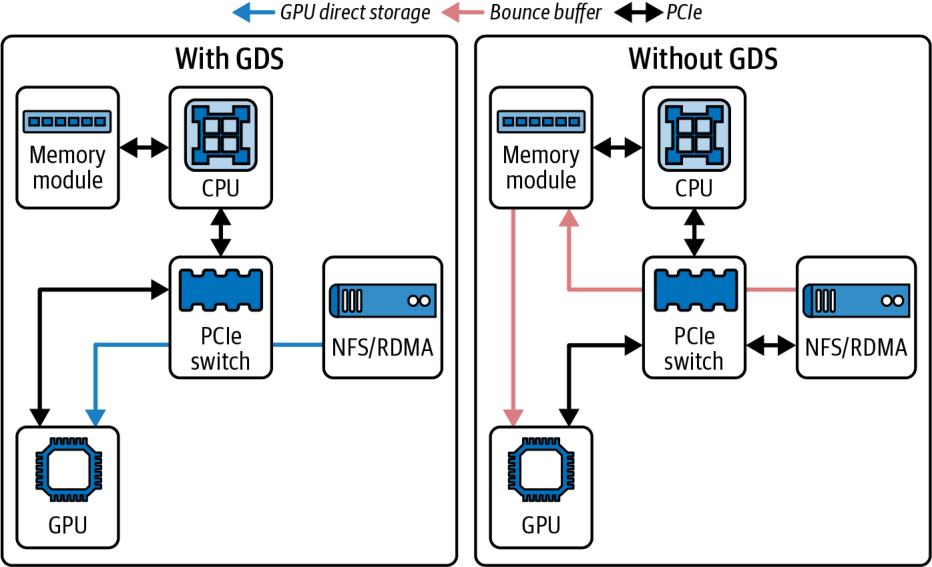
\includegraphics[width=\linewidth]{figs/fig5-1.png}\\
    {\scriptsize Figure 5-1. VAST Data's network architecture with GDS (left) vs.\ without (right)}
    \column{0.43\textwidth}
    \begin{itemize}\small
      \item Right: traditional \kw{staged DMA} --- the pink path copies through host memory.
      \item Left: \kw{direct GPU pull} over the PCIe switch --- host memory copies gone,
            CPU utilization down.
      \item VAST reports: \kw{+20\%} read throughput on an A100;
            \kw{+30\%+} on an H100 --- higher NIC bandwidth = greater CPU burden removed.
      \item Book caveat: \kw{validate on your workload} --- uplift varies with I/O size,
            queue depth, NIC generation, filesystem.
    \end{itemize}
  \end{columns}
  \pe{how much the shortcut saves depends on how congested the front office was --- measure \kw{your} building, not the vendor's.}
\end{frame}

% ================================================================ 10
\begin{frame}{Using GDS in Practice: the cuFile API}
  \begin{columns}[t]
    \column{0.52\textwidth}
    \begin{itemize}\small
      \item Applications read through CUDA's \kw{cuFile} library: \kw{\texttt{cuFileRead}}
            works on regular \kw{POSIX file descriptors}; automatic buffer alignment;
            the \kw{nvidia-fs} kernel driver orchestrates the DMA.
      \item Async variants \kw{\texttt{cuFileReadAsync} / \texttt{cuFileWriteAsync}} put storage
            I/O \kw{on CUDA streams} (Chapter 11) --- overlap and pipelining.
      \item \kw{Pinned host memory is not used} in the storage$\to$GPU path; cuFile registers
            \kw{GPU device buffers} instead.
    \end{itemize}
    \column{0.44\textwidth}
    \begin{block}{Requirements and supported stacks}
      \small Modern NVIDIA GPU + drivers + CUDA toolkit; DMA-capable storage stack:
      local NVMe / NVMe-oF on \kw{XFS/EXT4 with \texttt{O\_DIRECT}}, \kw{NFS over RDMA},
      and parallel filesystems integrating nvidia-fs (\kw{BeeGFS, WekaFS, VAST, IBM Storage Scale}).
    \end{block}
    \begin{itemize}\small
      \item Book tip: use \kw{\texttt{O\_DIRECT}} when possible; cuFile tolerates non-\texttt{O\_DIRECT}
            descriptors, but \kw{misalignment can cost extra copies}.
    \end{itemize}
  \end{columns}
  \pe{one library call, and the forklift route is booked end to end --- as long as the loading dock (filesystem) speaks the same protocol.}
\end{frame}

% ================================================================ 11
\begin{frame}{When Does GDS Actually Help?}
  \begin{columns}[t]
    \column{0.50\textwidth}
    \begin{block}{The honest answer (book)}
      \small If the CPU was \kw{easily handling} the transfers, GDS may not change
      throughput much --- but it still \kw{lowers CPU usage}, freeing cores for
      preprocessing. If the CPU is \kw{saturated with memcpys}, GDS \kw{helps a lot}.
    \end{block}
    \begin{itemize}\small
      \item Worked example: 1{,}000 batches/s $\times$ 1 MB $=$ \kw{1 GB/s}. Copying that
            through the CPU eats \kw{a few cores}; with GDS the GPU pulls it directly ---
            at higher rates or thousands of GPUs, the effect compounds.
    \end{itemize}
    \column{0.46\textwidth}
    \begin{itemize}\small
      \item Training is \kw{overwhelmingly read-heavy} --- most GDS gains are measured on
            reads.
      \item Fast \kw{checkpoint writes} matter too: RDMA-accelerated \kw{writes} require
            filesystem support --- e.g., \kw{WekaFS} ships GDS-aware plugins for both
            read and write paths.
      \item Vendor ecosystem (WekaIO, DDN, VAST, Cloudian\ldots) means GDS often works
            \kw{out of the box} on enterprise NAS / parallel filesystems.
    \end{itemize}
  \end{columns}
  \pe{the shortcut pays most when the office clerk was the queue --- and even when it isn't faster, the clerk is now free to do other work.}
\end{frame}

% ================================================================ 12
\begin{frame}[fragile]{Measuring It: gdsio Before and After}
  \begin{columns}[t]
    \column{0.56\textwidth}
\begin{lstlisting}[language=bash]
# Before: storage -> CPU memory (CPU path, -x 2)
$ /usr/local/cuda/gds/tools/gdsio \
    -f /mnt/data/large_file \
    -d 0 -w 4 -s 10G -i 1M -I 0 -x 2
Total Throughput: 8.0 GB/s   Avg Latency: 1.25 ms

# After: storage -> GPU memory via GDS (-x 0)
$ /usr/local/cuda/gds/tools/gdsio \
    -f /mnt/data/large_file \
    -d 0 -w 4 -s 10G -i 1M -I 0 -x 0
Total Throughput: 9.6 GB/s   Avg Latency: 1.00 ms
\end{lstlisting}
    {\footnotesize Same file, same workers/size/IO-size; only the \kw{transfer selector}
     (\texttt{-x}) changes --- compare paths consistently.}
    \column{0.40\textwidth}
    {\small\setlength{\tabcolsep}{4pt}
    \begin{tabular}{@{}lll@{}}
      \toprule
      \textbf{Path} & \textbf{Thpt} & \textbf{Latency} \\
      \midrule
      Storage $\to$ CPU & 8.0 GB/s & 1.25 ms \\
      Storage $\to$ GPU & \kw{9.6 GB/s} & \kw{1.00 ms} \\
       & (+20\%) & ($-$20\%) \\
      \bottomrule
    \end{tabular}}\\[4pt]
    {\small Table 5-1. \kw{gdsio} ships under \texttt{/usr/local/cuda/gds/tools} --- benchmark
    \kw{your} disk-to-GPU path before and after enabling GDS, while also freeing the CPU
    cycles previously spent in host buffers.}
  \end{columns}
  \pe{one tool, two flags, a clean 20\% verdict --- run it before you argue about architecture.}
\end{frame}

% ================================================================ 13
\begin{frame}{Checkpointing GPU State with cuda-checkpoint\ {\normalsize *}}
  \bridge{* A sidebar in the storage story: snapshotting a whole CUDA process, not writing model checkpoints.}
  \begin{columns}[t]
    \column{0.52\textwidth}
    \begin{itemize}\small
      \item \kw{cuda-checkpoint} + a CPU checkpointer (\kw{CRIU}) snapshot a \kw{running
            CUDA process}: lock CUDA entry points, \kw{drain outstanding work}, copy device
            memory \kw{to host}, release the GPU.
      \item Driver API: \texttt{cuCheckpointProcess\{Lock, Checkpoint, Restore, Unlock\}}.
            Restore needs persistence mode; can \kw{remap to different GPUs} of the same
            chip type.
      \item Suspend time $\approx$ \kw{device-memory image size $\div$ host-link bandwidth}
            --- verify with Nsight Systems markers.
    \end{itemize}
    \column{0.44\textwidth}
    \begin{block}{Two clarifications (book notes)}
      \small
      \begin{itemize}\small
        \item \kw{Not} a GDS path: device memory goes \kw{GPU $\to$ host} first;
              CRIU then persists the process image.
        \item \kw{Orthogonal} to framework checkpoints (PyTorch state-dicts) ---
              use it to \kw{complement, not replace} them: fault tolerance,
              preemption, migration of long-running jobs.
      \end{itemize}
    \end{block}
  \end{columns}
  \pe{it freezes the whole workshop mid-shift so it can reopen elsewhere --- different from photocopying the blueprints (model checkpoints).}
\end{frame}

% ================================================================ 14
\begin{frame}{DeepSeek's Fire-Flyer File System (3FS): Codesigning Storage for AI}
  \begin{columns}[c]
    \column{0.50\textwidth}
    \begin{itemize}\small
      \item Born from one observation: AI does \kw{massive random reads} --- read
            caching is \kw{counterproductive}. 3FS: \kw{no cache, direct I/O},
            straight to NVMe.
      \item Four components --- cluster manager, metadata service, storage service, client ---
            over an \kw{RDMA fabric} (InfiniBand/RoCE).
      \item Reported: \kw{6.6 TB/s} aggregate reads on 68 nodes (+1.4 TB/s background);
            up to \kw{7.3 TB/s} --- vs.\ Ceph's $\sim$1.1 TB/s on similar hardware.
      \item Book caveat: building your own FS is a \kw{big investment} --- most teams
            should start from existing systems (next part).
    \end{itemize}
    \column{0.46\textwidth}
    \centering
    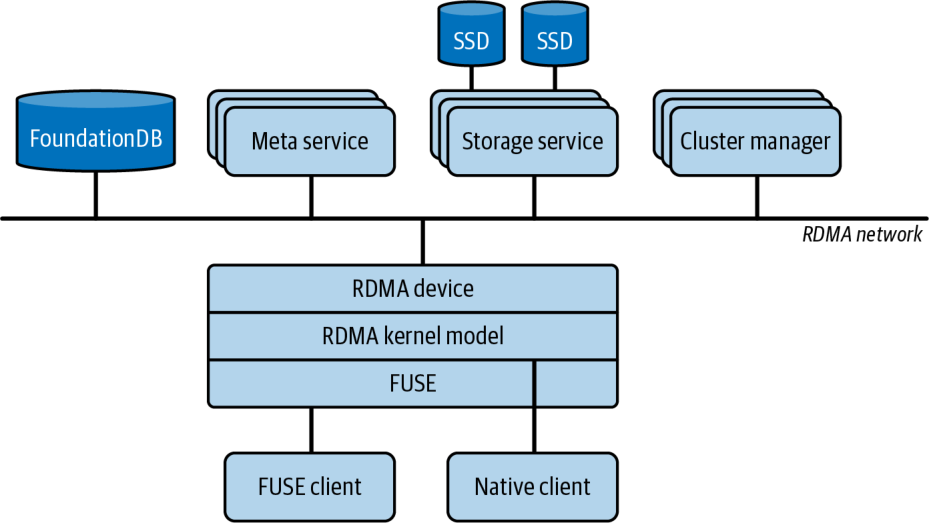
\includegraphics[width=0.78\linewidth]{figs/fig5-2.png}\\
    {\scriptsize Figure 5-2. Components of DeepSeek's Fire-Flyer File System (3FS)}\\[3pt]
    \begin{block}{FUSE caveat (book warning)}
      \footnotesize A \kw{FUSE} (user-space) filesystem \kw{cannot} deliver a GDS path ---
      GDS needs \kw{kernel-level} \texttt{O\_DIRECT} integration (NVMe/NVMe-oF, BeeGFS,
      WekaFS, IBM Storage Scale, VAST).
    \end{block}
  \end{columns}
  \pe{DeepSeek rebuilt the warehouse around how AI shops: random grabs, no shelves, forklifts only.}
\end{frame}

% ================================================================ 15
\begin{frame}[fragile]{Part III --- NFS: Simple to Set Up, Simple to Saturate}
  \bridge{Custom filesystems are the exception. What do the rest of us mount?}
  \begin{columns}[t]
    \column{0.50\textwidth}
    \begin{itemize}\small
      \item One shared NFS server = every node reads the same place --- convenient, and a
            \kw{throughput bottleneck} once many nodes read at once.
      \item If you must use NFS: \kw{multiple fast NICs}, or \kw{multiple servers} each
            holding a partition of the dataset; NVMe (even RAID 0) underneath.
      \item Book verdict: NFS \kw{only for modest scale} (a few nodes) --- larger clusters
            want parallel filesystems or cloud caches (next page).
    \end{itemize}
    \column{0.46\textwidth}
    \begin{block}{Client-side tuning that actually matters}
      \small \kw{rsize/wsize} at the max (1 MB); kill access-time writes; cache attributes:
    \end{block}
\begin{lstlisting}[language=bash]
mount -o rsize=1048576,wsize=1048576,\
noatime,async,actimeo=60,lookupcache=pos \
  nfs-server:/data /mnt/data
\end{lstlisting}
    {\footnotesize 1 MiB requests + \texttt{noatime} + 60 s attribute/directory caching ---
     simple tweaks that vastly cut per-request overhead on large shared datasets.}
  \end{columns}
  \pe{one shop counter serving the whole city works fine --- until the whole city shows up at once.}
\end{frame}

% ================================================================ 16
\begin{frame}{Parallel Filesystems and Object Stores}
  \begin{columns}[t]
    \column{0.50\textwidth}
    \begin{block}{Parallel FS: stripe for bandwidth}
      \small Lustre serves data from multiple \kw{OSTs} (object storage targets).
      \kw{Stripe} large files across OSTs (\texttt{lfs setstripe}, e.g.\ 4--8):
      4 OSTs $\times$ 500 MB/s $=$ \kw{2 GB/s} theoretical read peak per file.
    \end{block}
    \begin{itemize}\small
      \item Monitor during training (\kw{lmt}, vendor dashboards): a few \kw{hot} storage
            nodes usually means a \kw{sharding imbalance} --- find out why.
    \end{itemize}
    \column{0.46\textwidth}
    \begin{block}{Object stores: stage or cache}
      \small Naive S3 reads during training are slow. Either \kw{stage to local NVMe}
      before training (\kw{s5cmd}, AWS C++ SDK --- highly parallel tools), or put a
      \kw{cache layer} on top (Amazon FSx for Lustre over S3).
    \end{block}
    \begin{itemize}\small
      \item Streaming directly? Use \kw{large range-GETs}, multithreaded.
      \item Book tip: \kw{verify} the cache's performance uplift actually justifies its
            cost --- work with the provider if numbers disappoint.
    \end{itemize}
  \end{columns}
  \pe{ten loading docks beat one; and if the goods live overseas (S3), either ship ahead of time or rent a local depot.}
\end{frame}

% ================================================================ 17
\begin{frame}{Two Blunt but Effective Levers: Replicate and Compress}
  \begin{columns}[t]
    \column{0.48\textwidth}
    \begin{block}{Replicate the dataset to every node}
      \small Brute force: copy the \kw{whole dataset} onto each node's disk ---
      \kw{zero network reads}, immediate win, at the cost of storage.
      Common and very effective when node storage allows.
    \end{block}
    \column{0.48\textwidth}
    \begin{block}{Store compressed, decompress on the fly}
      \small JPEGs, compressed Arrow/Parquet: trade \kw{I/O bandwidth} for CPU/GPU cycles ---
      reasonable exactly when \kw{I/O is the bottleneck} and compute is idle.
    \end{block}
  \end{columns}
  \medskip
  \begin{itemize}\small
    \item Decode on the GPU: \kw{nvJPEG} for images; Blackwell's on-die
          \kw{Decompression Engine} handles \kw{LZ4, Snappy, Deflate} in-pipeline ---
          SMs stay free for compute kernels. \kw{Favor these formats} for I/O-bound work.
    \item \kw{NVLink-C2C} ($\sim$900 GB/s bidirectional) keeps CPU-assisted stages from
          becoming the new bottleneck.
    \item The balance test: if \kw{decompression time replaces I/O} as the bottleneck,
          the compression wasn't worth it.
  \end{itemize}
  \pe{either give every workshop its own copy of the catalog, or ship the catalog vacuum-packed --- just make sure unpacking isn't slower than shipping was.}
\end{frame}

% ================================================================ 18
\begin{frame}{Monitoring Storage I/O: the Toolbox}
  \begin{columns}[t]
    \column{0.50\textwidth}
    \begin{block}{Host OS tools}
      \small \kw{iostat, iotop, nvme-cli, perf, eBPF} + vendor dashboards ---
      queues, latencies, read-ahead effects, cache hit ratios; are local NVMe or the
      network links to NAS/object storage \kw{saturated}?
    \end{block}
    \begin{itemize}\small
      \item \kw{DCGM} (Data Center GPU Manager) adds GPU-side I/O statistics ---
            together they expose \kw{GPU starvation due to I/O}.
    \end{itemize}
    \column{0.46\textwidth}
    \begin{block}{GDS-aware tracing}
      \small Nsight Systems with \kw{\texttt{--trace=gds}} captures \kw{cuFile API activity}
      on the timeline; enable cuFile static tracepoints via \texttt{/etc/cufile.json}.
    \end{block}
    \begin{itemize}\small
      \item Caveat: kernel-mode counters for NVMe \kw{peer-to-peer DMA} aren't exposed in
            Nsight Systems and may be missing on some GDS stacks.
    \end{itemize}
  \end{columns}
  \pe{same rule as every chapter: no verdict without a measurement --- the disk, the NIC, and the GPU each get their own gauge.}
\end{frame}

% ================================================================ 19
\begin{frame}{Whose Fault Is the Idle GPU? A Two-Timer Decomposition}
  \begin{columns}[t]
    \column{0.52\textwidth}
    \begin{itemize}\small
      \item In PyTorch, timing \kw{\texttt{next(data\_iterator)}} measures \kw{total GPU idle
            time waiting for a batch} --- prefetching + H2D copy included, not just Python.
      \item Split it in two:
            \kw{(1) Python cost} --- set \kw{\texttt{num\_workers=0}} and time the bare
            iterator pull;
            \kw{(2) H2D copy cost} --- wrap \texttt{.to("cuda")} in \kw{CUDA events}, or read
            the \kw{Copy lanes} in Nsight Systems.
      \item Compare both against total idle time $\Rightarrow$ speed up the \kw{Python
            pipeline} (workers, simpler transforms) or the \kw{transfer path}
            (pinned memory, interconnect, GDS).
    \end{itemize}
    \column{0.44\textwidth}
    \begin{block}{Why this matters (book example)}
      \small GPUs waiting \kw{30\%} of the time for data $\Rightarrow$ throughput capped by
      I/O. After tuning: waiting \kw{5\%} --- training steps/s up \kw{proportionally}.
    \end{block}
    \begin{itemize}\small
      \item Storage tuning = killing many small inefficiencies (5 ms here, a small
            buffer there) --- at scale they \kw{add up}.
    \end{itemize}
  \end{columns}
  \pe{first clock \kw{how long} the crew stands idle; then split the blame between the kitchen (Python) and the delivery van (H2D copy).}
\end{frame}

% ================================================================ 20
\begin{frame}{Part IV --- The Data Pipeline: The Last Mile to the GPU}
  \bridge{Storage delivers bytes; someone still has to turn bytes into batches.}
  \begin{columns}[c]
    \column{0.55\textwidth}
    \begin{itemize}
      \item Typical loading path: \kw{read} from storage $\to$ \kw{decode/deserialize}
            (JSON, JPEG) $\to$ \kw{transform} (tokenize, crop) $\to$ \kw{collate} into batches.
      \item These steps are CPU-intensive --- but compute-heavy ones can be
            \kw{offloaded to the GPU}.
      \item Goal: GPUs \kw{never idle} waiting for data, with the \kw{right amount} of CPU
            work running in parallel.
    \end{itemize}
    \column{0.42\textwidth}
    \begin{block}{Perspective (book)}
      \small A poorly tuned input pipeline can waste \kw{50\%} of GPU time; algorithmic
      tweaks often buy only \kw{a few percent}. Optimizing the pipeline frequently
      \kw{beats model-level cleverness}.
    \end{block}
  \end{columns}
  \pe{the last mile decides the delivery date --- a warehouse full of parts feeds nothing if the kitting bench is slow.}
\end{frame}

% ================================================================ 21
\begin{frame}{DataLoader Essentials: the Five Knobs}
  \begingroup\footnotesize\setlength{\tabcolsep}{4pt}\renewcommand{\arraystretch}{1.2}
  \begin{tabular}{@{}lll@{}}
    \toprule
    \textbf{Knob} & \textbf{What it does} & \textbf{Guidance} \\
    \midrule
    \texttt{num\_workers} & parallel fetch+preprocess \kw{processes} (GIL-free) & empirical; watch CPU + disk \\
    \texttt{pin\_memory=True} & page-locked host buffers & enables real async H2D \\
    \texttt{non\_blocking=True} & async \texttt{.to(device)} copies & pairs with pinned memory \\
    \texttt{persistent\_workers=True} & workers survive across epochs & kills respawn overhead \\
    \texttt{prefetch\_factor} & batches queued per worker (default 2) & 4--8 for bursty I/O \\
    \bottomrule
  \end{tabular}\endgroup
  \medskip
  \begin{itemize}\small
    \item Too few workers $\Rightarrow$ idle GPU; too many $\Rightarrow$ contention for CPU
          cores and I/O bandwidth. Aim for \kw{$\sim$100\% disk throughput, headroom on CPU}.
    \item High-core CPUs (72-core \kw{Grace}) can host more workers --- mind diminishing returns.
    \item Scaling out GPUs? \kw{Scale the pipeline too}: each rank reads its own shard; aggregate
          loading work \kw{grows with cluster size} --- or the bottleneck shifts to ingestion.
    \item Set a high \kw{\texttt{ulimit -l}} (memlock) so large pinned buffers can allocate.
  \end{itemize}
  \pe{five dials on one machine --- and more chefs (GPUs) always means more prep cooks (workers).}
\end{frame}

% ================================================================ 22
\begin{frame}[fragile]{The Overlap in Code: Pinned Memory + Prefetch + Streams}
  \begin{columns}[t]
    \column{0.56\textwidth}
\begin{lstlisting}[language=Python]
loader = DataLoader(
    dataset, batch_size=B,
    num_workers=8, pin_memory=True,
    persistent_workers=True, prefetch_factor=4)

copy_stream = torch.cuda.Stream()
compute_stream = torch.cuda.current_stream()
for batch in loader:
    with torch.cuda.stream(copy_stream):
        batch_gpu = batch.to(device, non_blocking=True)
    # H2D must finish before compute uses it
    with torch.cuda.stream(compute_stream):
        torch.cuda.current_stream().wait_stream(copy_stream)
        outputs = model(batch_gpu)
\end{lstlisting}
    \column{0.40\textwidth}
    \begin{itemize}\small
      \item 8 workers, each keeping \kw{4 batches} queued in \kw{pinned} memory
            (\texttt{num\_workers} $\times$ \texttt{prefetch\_factor} total).
      \item Pinned source $\Rightarrow$ \texttt{non\_blocking} copy uses \kw{DMA}:
            while the GPU computes batch $N$, batch $N{+}1$ is \kw{already transferring}.
      \item Without pinning, memory is pinned \kw{on the fly per transfer} ---
            latency you didn't order.
    \end{itemize}
  \end{columns}
  \pe{the prep station always keeps the next tray loaded --- the chef never looks up between dishes.}
\end{frame}

% ================================================================ 23
\begin{frame}{Avoid Python Bottlenecks; Profile the Loader in Isolation}
  \begin{columns}[t]
    \column{0.50\textwidth}
    \begin{itemize}\small
      \item Red flag: \kw{pure-Python loops} tokenizing lines one by one. Vectorize, or use
            \kw{Rust/C++-backed} libraries (Hugging Face Tokenizers, TorchText) --- Python is
            just the interface.
      \item Prefer \kw{batched transforms}: collate first (custom \texttt{collate\_fn}), then
            transform \kw{whole tensors} --- some ops must stay per-sample; know your workload.
      \item Hidden bottlenecks sneak in easily: \kw{debug logging}, expensive CPU transforms
            --- often visible \kw{only under load}.
    \end{itemize}
    \column{0.46\textwidth}
    \begin{block}{Baseline the loader alone}
      \small Time how long the DataLoader takes to produce \kw{100 batches} with all
      GPU work disabled; compare with target iteration time and measured GPU-idle time.
      Loader too slow? Fewer logs, simpler transforms, \kw{more workers}.
    \end{block}
    \begin{itemize}\small
      \item Caveat (book note): disabling GPU work also removes \kw{kernel-launch overhead},
            so isolated loader throughput reads \kw{lower} than in a real run --- still useful,
            just remember it.
    \end{itemize}
  \end{columns}
  \pe{time the prep kitchen with the dining room closed --- just remember service adds its own noise when you reopen.}
\end{frame}

% ================================================================ 24
\begin{frame}{Multimodal Preprocessing on the GPU: NVIDIA DALI}
  \begin{columns}[t]
    \column{0.50\textwidth}
    \begin{itemize}\small
      \item \kw{DALI} moves decoding/augmentation to the GPU (or optimized C++ CPU code):
            JPEG decode, random crop, resize, normalize --- using the GPU's
            \kw{media-acceleration hardware}.
      \item Declarative \kw{static graph}: subclass \texttt{Pipeline}, declare ops in
            \texttt{define\_graph()}; DALI handles execution, prefetching, threading.
      \item Book example: CPU at \kw{800\%} (8 cores) with a stalling GPU $\to$ with DALI,
            CPU at \kw{200\%} while the GPU decodes \kw{concurrently with compute}.
    \end{itemize}
    \column{0.46\textwidth}
    \begin{block}{The placement pitfall}
      \small Using DALI \kw{only to decode}, then handing pixels \kw{back to the CPU} for
      augmentation adds \kw{host--device--host} copies that can \kw{negate the gains}.
    \end{block}
    \begin{itemize}\small
      \item Alternative (book tip): \kw{fuse} GPU-friendly preprocessing into your GPU graph
            with TorchVision / TensorRT / custom CUDA kernels --- may beat DALI end to end.
      \item Benchmark \kw{three ways}: CPU-only vs.\ DALI vs.\ fully fused GPU graph.
    \end{itemize}
  \end{columns}
  \pe{moving the chopping board next to the stove helps only if the food doesn't travel back to the pantry between steps.}
\end{frame}

% ================================================================ 25
\begin{frame}{Prepare Data Offline: NVIDIA NeMo Curator}
  \begin{columns}[t]
    \column{0.52\textwidth}
    \begin{itemize}\small
      \item \kw{NeMo Curator} (open source) prepares \kw{multiterabyte LLM datasets} ahead of
            training: cleansing, tokenizing, shuffling, \kw{deduplication}, quality filtering
            --- distributed across \kw{multiple GPUs/nodes}.
      \item Packs data into \kw{few large files}; NeMo training reads memory-mappable
            \kw{.bin + .idx}; Curator I/O is sharded JSONL/Parquet.
      \item Can also generate \kw{synthetic data} to augment increasingly scarce human data.
    \end{itemize}
    \column{0.44\textwidth}
    \begin{block}{Why offline prep wins}
      \small Training becomes \kw{mostly forward/backward passes}: consistent, evenly
      sized, padded inputs; \kw{no on-the-fly tokenization}, no millions of small files.
    \end{block}
    \begin{itemize}\small
      \item Book tip: store \kw{N differently shuffled copies} to avoid runtime shuffling
            across N epochs --- disk space for speed.
      \item ``\kw{Almost never} train with raw text.'' NeMo loading still runs on
            \kw{CPUs} --- combine with \kw{GDS} to bypass CPU I/O.
    \end{itemize}
  \end{columns}
  \pe{do the mise en place the night before --- during service you only plate.}
\end{frame}

% ================================================================ 26
\begin{frame}{Part V --- The Continuous Profiling and Tuning Loop}
  \bridge{Everything so far is a one-time fix. Performance, though, is a feature that needs regression testing.}
  \begin{columns}[t]
    \column{0.52\textwidth}
    \begin{enumerate}\small
      \item \kw{Establish a baseline}: single GPU $\to$ one node $\to$ multinode, tracking
            samples/s. N GPUs should give \kw{$\sim$N$\times$}; 8 GPUs at 5$\times$ =
            \kw{62.5\% efficiency} --- quantify the gap.
      \item \kw{Profile the multi-GPU run} (\kw{nsys}): GPUs idle \kw{during all-reduce}
            $\Rightarrow$ communication; idle \kw{at iteration start} $\Rightarrow$ data
            loading; check CPU timelines and sync points too.
      \item \kw{Zoom into kernels} (\kw{ncu}) when one op underperforms --- book example: an
            NCCL kernel at \kw{60\% SM utilization} over PCIe; on NVLink, \kw{90\%}.
    \end{enumerate}
    \column{0.44\textwidth}
    \begin{block}{The loop}
      \centering\small Run $\to$ Measure $\to$ Tune $\to$ Run $\to$ Measure $\to$ Tune $\to\cdots$
    \end{block}
    \begin{itemize}\small
      \item Every kernel verdict lands in one of three bins: \kw{network-bandwidth,
            memory-bandwidth, or compute bound}.
      \item It's much easier to \kw{maintain} good performance than to \kw{regain} it later.
    \end{itemize}
  \end{columns}
  \pe{treat performance like a test suite: it either passes tonight, or you find out tomorrow which commit broke it.}
\end{frame}

% ================================================================ 27
\begin{frame}{Identify the Cause, Fix One Thing, Remeasure}
  \begin{columns}[t]
    \column{0.50\textwidth}
    \begin{block}{Map bottleneck $\to$ hypotheses $\to$ fixes}
      \small
      \begin{itemize}\small
        \item \kw{Network}: GPUDirect RDMA; bigger messages;
              \texttt{NCCL\_NSOCKS\_PERTHREAD}; NUMA-aware binding.
        \item \kw{Straggler GPU}: data imbalance or extra logging on one rank ---
              move it off the critical path.
        \item \kw{CPU/data}: more workers, DALI offload, more offline preprocessing.
        \item \kw{Sync}: remove stray \texttt{torch.cuda.synchronize()} / barriers (Ch.\ 13).
      \end{itemize}
    \end{block}
    \column{0.46\textwidth}
    \begin{itemize}\small
      \item \kw{Change 1--2 things at a time}, then remeasure --- otherwise you can't
            credit the right fix.
      \item \kw{Updates shift optima}: new NCCL/CUDA/PyTorch can help --- rerun the
            workflow after every upgrade.
      \item \kw{Automate}: nightly profiling runs, dashboards, alerts on utilization drops.
      \item \kw{Document} tacit knowledge in code/config ---
            ``\texttt{NCCL\_SOCKET\_NTHREADS=2} gave +10\% on this cluster.''
    \end{itemize}
  \end{columns}
  \pe{tune like a scientist: one variable, one measurement, one written-down conclusion.}
\end{frame}

% ================================================================ 28
\begin{frame}{Communication- or Compute-Bound? The Batch-Size Experiment}
  \begin{columns}[t]
    \column{0.52\textwidth}
    \begin{itemize}\small
      \item Setup: gradient all-reduce uses \kw{60 GB/s of a 100 GB/s NIC}. Clogged
            network, or slow GPUs?
      \item Key fact: all-reduce traffic scales with \kw{parameter count, not batch size}
            --- batch size varies \kw{compute} at \kw{fixed communication}.
      \item \kw{Halve the batch}: NIC stays at 60 GB/s $\Rightarrow$ \kw{network-bound};
            drops to 40 GB/s $\Rightarrow$ \kw{compute-bound} (GPUs starve the NIC).
      \item \kw{Double the batch} to confirm: NIC pinned at 60 $\Rightarrow$ communication
            limits; \kw{all-reduce share of time shrinks} $\Rightarrow$ compute limits.
    \end{itemize}
    \column{0.44\textwidth}
    \begin{block}{Read it like a roofline}
      \small Plot \kw{achieved GB/s} and \kw{\% time in communication} vs.\ batch size ---
      the plot shows where the ceiling is and \kw{which subsystem to tune}.
    \end{block}
    \begin{itemize}\small
      \item Nsight tip: long \kw{NCCL-wait} gaps between kernels $\Rightarrow$
            communication-bound; busy GPUs below expected FLOPS $\Rightarrow$
            memory- or compute-bound (ncu / PyTorch profiler).
    \end{itemize}
  \end{columns}
  \pe{hold the shipping volume constant and vary the workload --- whichever side refuses to move is your bottleneck.}
\end{frame}

% ================================================================ 29
\begin{frame}{Key Takeaways (the Book's Three)}
  \begin{columns}[t]
    \column{0.48\textwidth}
    \begin{block}{1 --- Scale the input pipeline with compute}
      \small More GPUs demand more storage bandwidth \kw{and} more loader parallelism ---
      or added GPUs give \kw{zero speedup}.
    \end{block}
    \begin{block}{2 --- Use the right tool for the job}
      \small \kw{NCCL} for collectives (training); \kw{NIXL} for point-to-point token
      streaming (inference); \kw{GPUDirect RDMA / GDS} remove the bounce buffer for
      network / storage; always \kw{DistributedDataParallel} over DataParallel.
    \end{block}
    \column{0.48\textwidth}
    \begin{block}{3 --- Profile end to end}
      \small The bottleneck is \kw{not obvious}: GPUs are compute-, communication-, or
      I/O-bound. Nsight Systems + Nsight Compute + PyTorch profiler + NCCL logs tell you
      \kw{which} --- then this chapter tells you what to do about it.
    \end{block}
    \begin{itemize}\small
      \item These libraries are \kw{purpose-built and heavily tuned} --- leverage them
            instead of reinventing the wheel.
    \end{itemize}
  \end{columns}
  \pe{feed the factory, take the shortcut past the front office, and never argue about the bottleneck --- measure it.}
\end{frame}

% ================================================================ 30
\begin{frame}{Conclusion and What's Next}
  \begin{block}{This chapter in one sentence}
    \kw{Fast data movement is as critical as raw compute} --- the fastest GPU in the world
    provides little benefit if it's constantly waiting for data from storage.
  \end{block}
  \begin{itemize}
    \item Storage is a \kw{foundational layer}: NVMe + GDS + tuned pipelines shorten
          training time and \kw{raise the rate of experimentation}.
    \item You \kw{don't need custom I/O solutions}: NVIDIA and the open source community ship
          highly tuned, purpose-built tools --- focus on your model, data, and application.
    \item Full-stack thinking continues: overlap communication/computation, use the fastest
          links available, keep every pipe full --- \kw{faster time-to-insight, better
          utilization, lower cost}.
    \item Next in the book: \kw{Chapter 6} --- GPU architecture, CUDA, and occupancy
          (covered in our previous session); the storage principles here stay relevant at
          \kw{every} layer above.
  \end{itemize}
  \medskip
  \centering\itshape Questions?
\end{frame}

% ================================================================ 31
\begin{frame}{References \& Further Reading}
  \begingroup\footnotesize
  \begin{enumerate}
    \item C.\ Fregly. \emph{AI Systems Performance Engineering} (O'Reilly, 2026), Chapter 5.
    \item NVIDIA. \emph{GPUDirect Storage Documentation} --- cuFile API reference,
          \texttt{gdsio} benchmarking guide, \texttt{cufile.json} configuration.
    \item NVIDIA. \emph{cuda-checkpoint} (GitHub) and CRIU --- Checkpoint/Restore in Userspace.
    \item DeepSeek. \emph{Fire-Flyer File System (3FS)} --- open source repository and
          Fire-Flyer AI-HPC paper (arXiv:2408.14158).
    \item NVIDIA. \emph{DALI Documentation} --- pipelines, GPU decode, framework integration.
    \item NVIDIA. \emph{NeMo Curator} --- documentation and GitHub repository.
    \item Linux kernel documentation --- \texttt{blk-mq}, I/O schedulers, \texttt{io\_uring};
          PyTorch docs --- \texttt{DataLoader}, \texttt{DistributedSampler}.
    \item VAST Data. \emph{GPUDirect Storage benchmark reports} (A100/H100 read-throughput uplifts).
  \end{enumerate}\endgroup
\end{frame}

\end{document}
